\section{Discussion}
\label{sec:discussion}
In this section we will present results from our experiments. We will look at cross dataset performance of our models, and look back at the results from human benchmarking (Section \ref{sec:human}) to see if our models hold up to the conclusions and resulting adjustments we made there. We also benchmark our models against the datasets we collected in section \ref{sec:data} and analyse the performance against multilingual datasets.

% \subsection{Cross Dataset Validation}
% \label{sec:cross_dataset}

% \begin{figure}
%     \centering
%     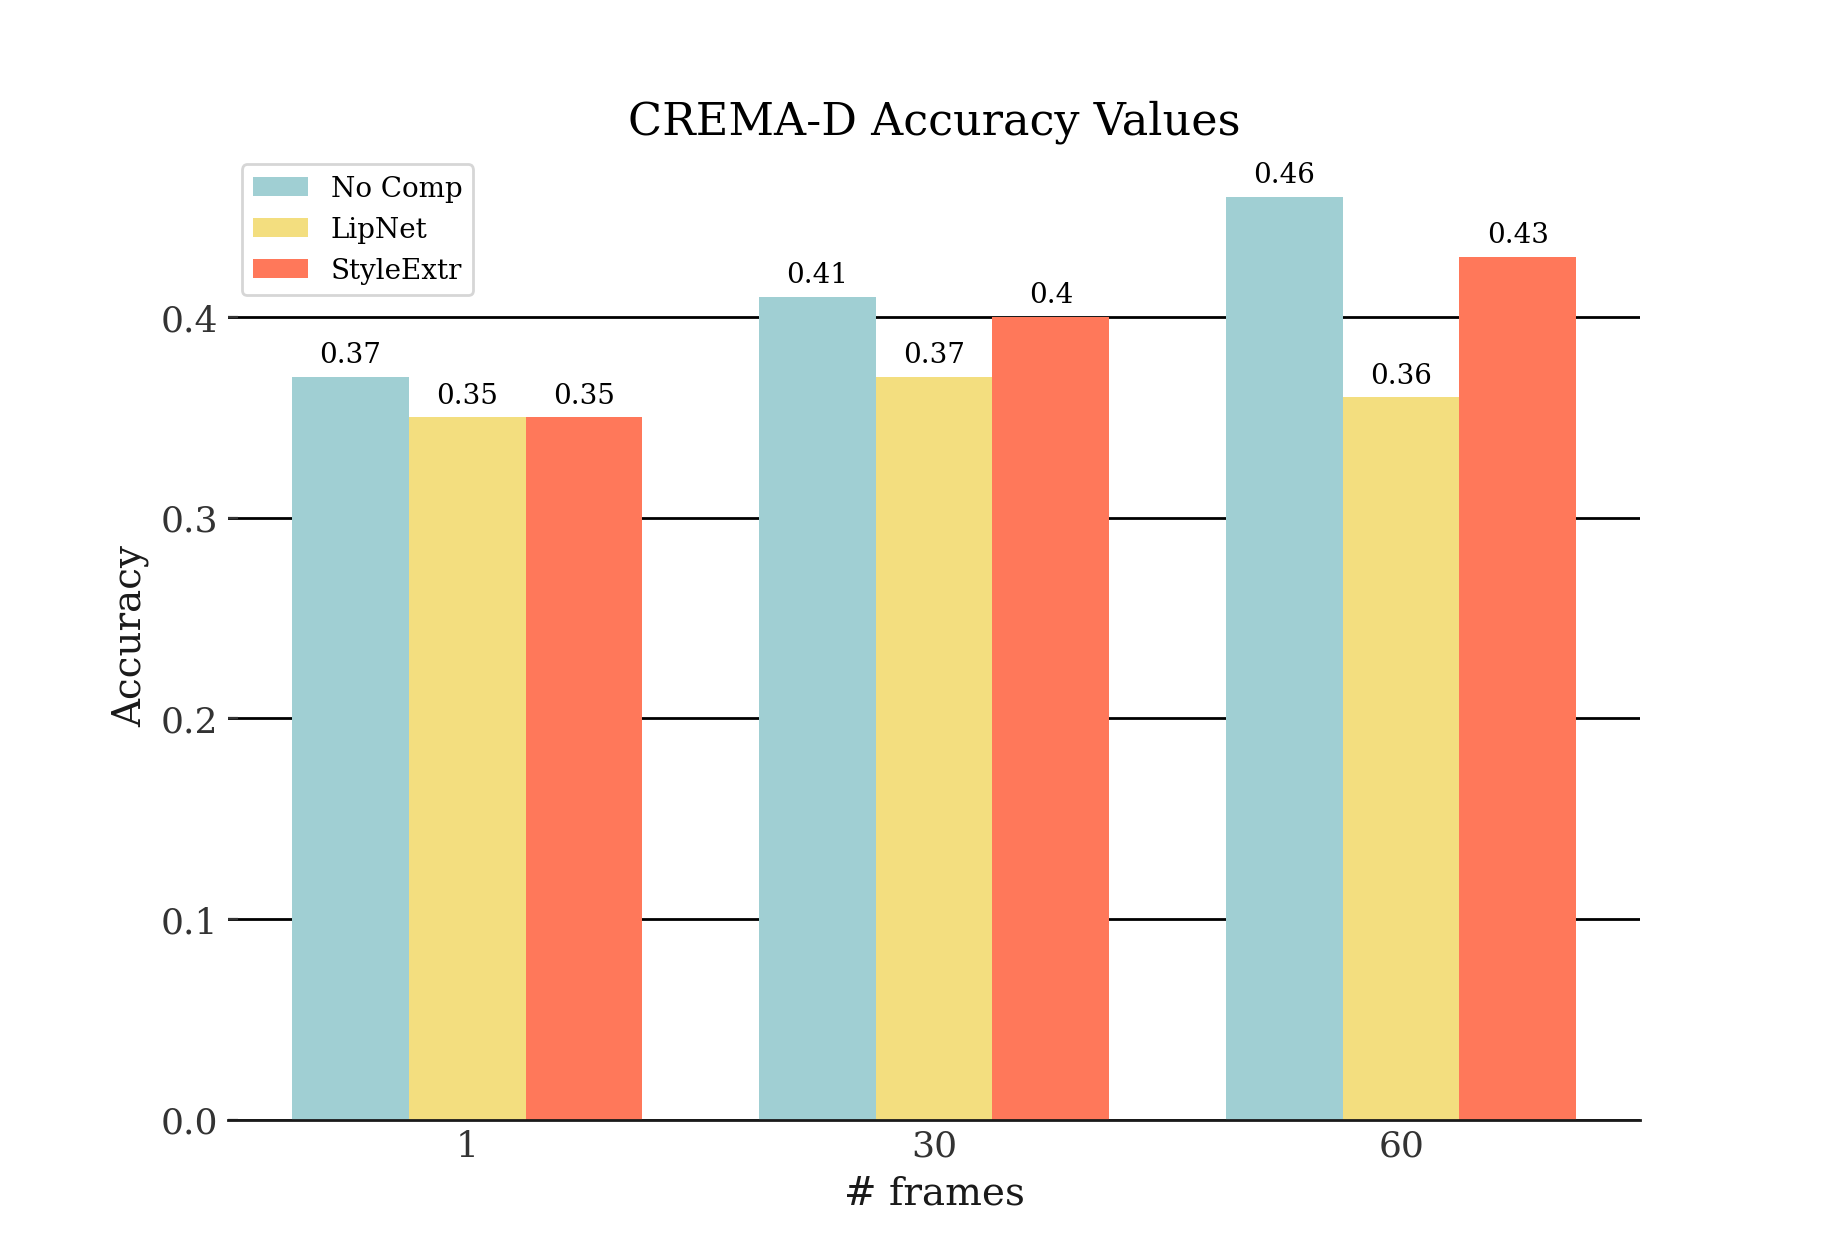
\includegraphics[width=0.8\textwidth]{res/CremaValidation.png}
%     \caption{Validation results of the our models on the CREMA-D corpus. A result for 90 frames was not possible since most videos in the CREMA-D database are not long enough.}
%     \label{fig:crema_val_lipnet}
% \end{figure}

% All our models on the FER section were trained on RAVDESS. An interesting question is if and how well the models generalize to other datasets, in this case CREMA-D. We ran validation on all our models using the CREMA-D corpus and compared the results \ref{fig:crema_val_lipnet}. We could not run the models trained on 90 frames since the videos in the CREMA-D database do not have enough frames.

% \subsubsection{General Results}
% Looking at the performance of the FER model, we see a continued trend for the importance of the existence and size of the temporal dimension. An increase in frame-window size from one to 60 improved the results by 24\%, or nine percentage points. An better performance can also be observed compared to the LipNet model. The FER model consistently performs better than its LipNet counterpart, up to 28\%, or ten percentage points. The LipNet model itself did not benefit from the temporal dimension. Its performance was between 35\% and 37\% throughout the different frame-window sizes. The style extractor model however also continued the trend of improvement with more temporal information. It also performs worse than the temporalized FER model, within a margin of one to three percentage points. 

% The performance of the style extractor compared to the LipNet model on domain shifts point to issues in using and training lexical compensators. A more robust and specialized lexical compensator produces better results than an off-the-shelve, tangentially related model. However, even the style extractor performed worse than the temporalized FER model. A combination of two models will produce compound errors, which can be managed by training on more diverse datasets.

% \subsubsection{Intensities}
% We also analysed the performance on CREMA-D based on the labelled intensity for each video (Figure \ref{fig:crema_intesities}). An interesting pattern emerges. At lower frames the StyleExtractor performs significantly better on \texttt{low} and \texttt{medium} intensity recordings compared to the other models. \texttt{High} and \texttt{low} intensity recordings are estimated more accurately than those of \texttt{medium} intensity. When increasing the frame-window size, the model without lexical compensation improves significantly. The models with compensators do not gain as much accuracy, especially the LipNet model which stays similar in accuracy throughout all frame-window sizes. These results are different from the ones in section \ref{sec:model_results}. On the RAVDESS dataset we saw a definitive increase in accuracy on higher intensity recordings. The RAVDESS corpus did not provide \texttt{low} intensity videos. Its \texttt{normal} intensity is comparable to the \texttt{medium} intensity of CREMA-D.


% \begin{figure}[!htb]
%     \centering
%     \begin{subfigure}[b]{0.45\textwidth}
%       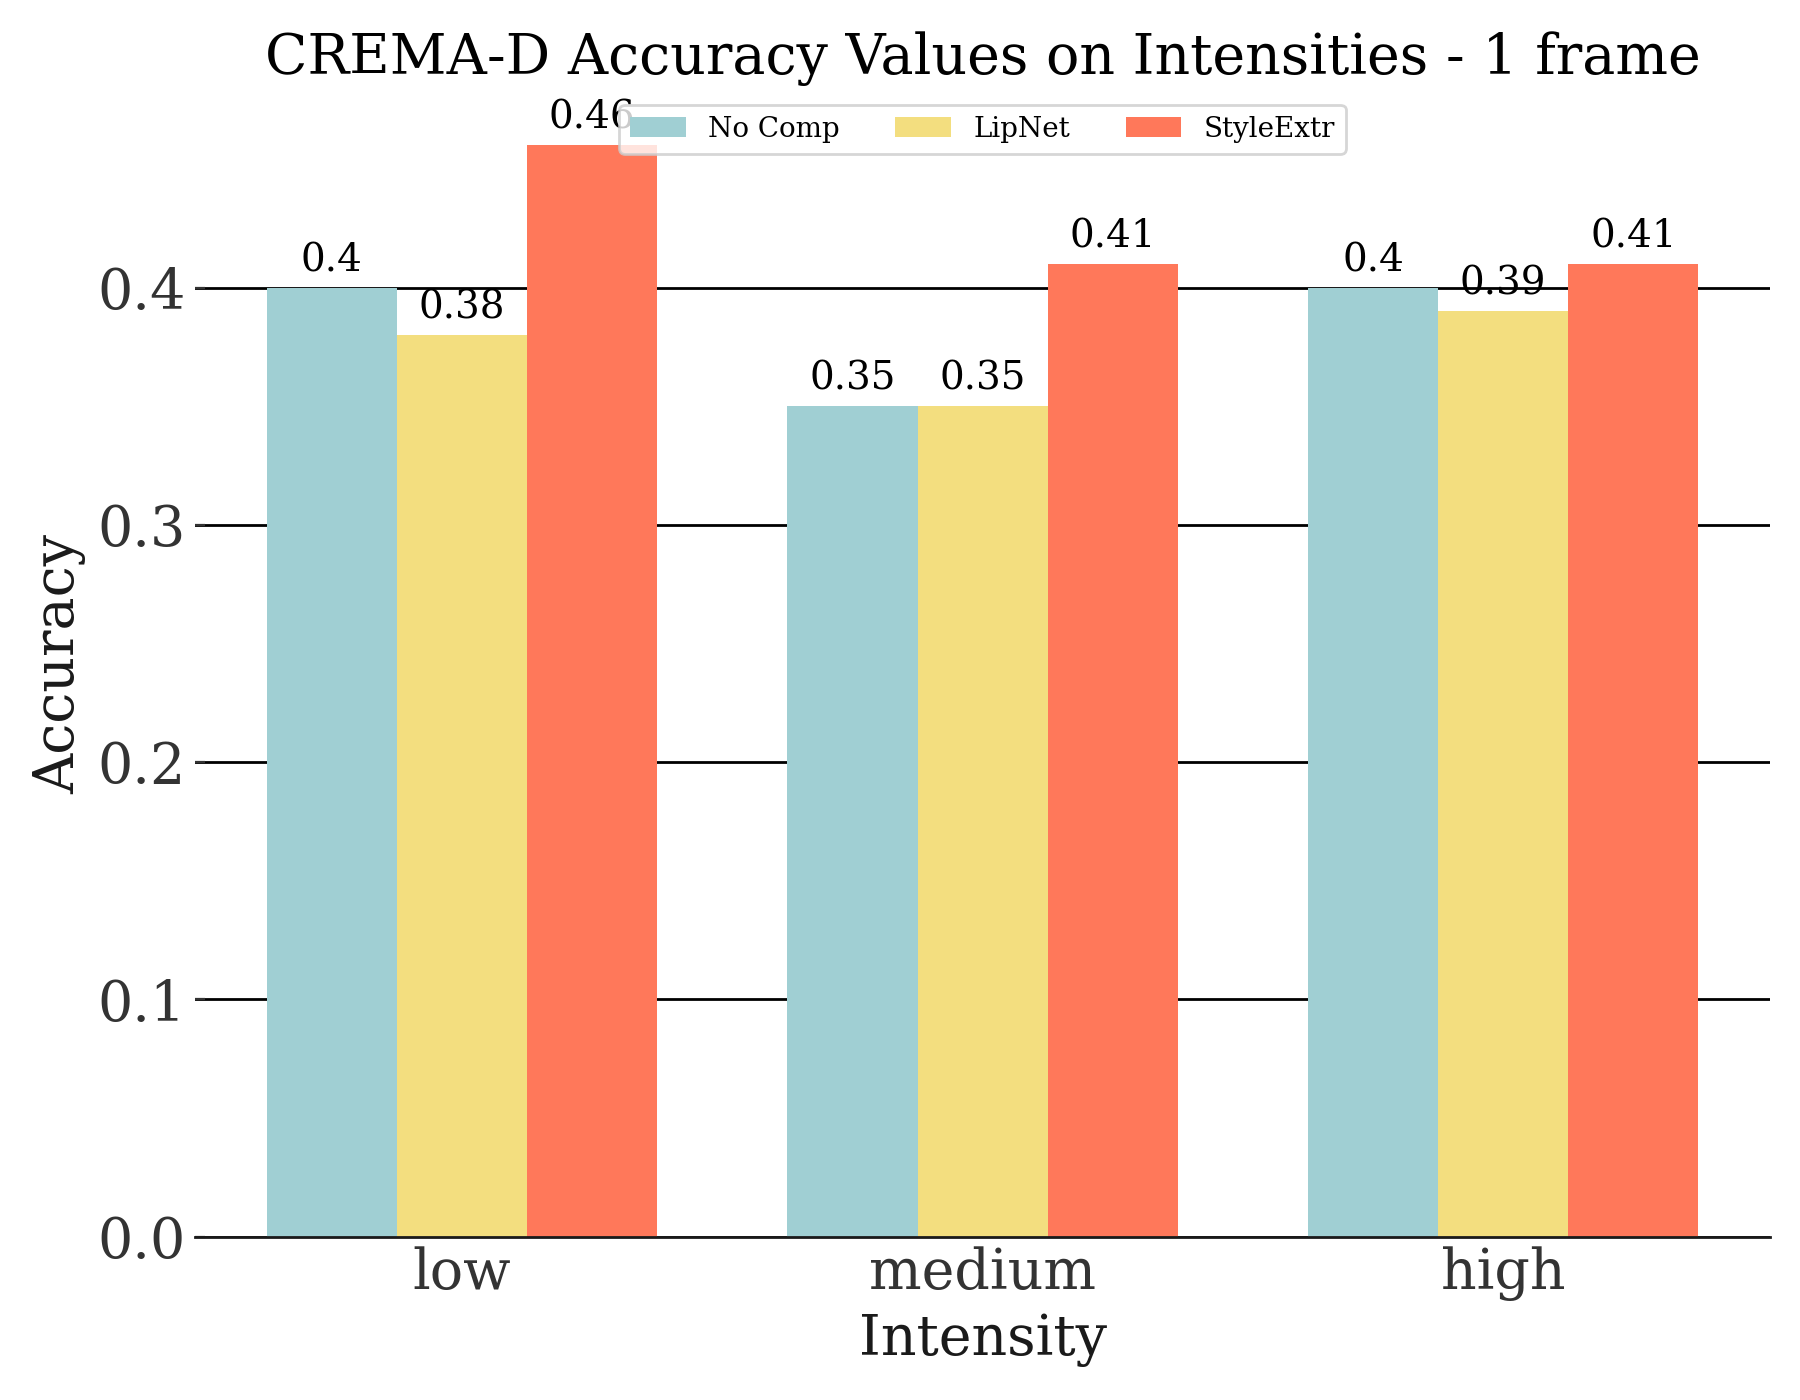
\includegraphics[width=\textwidth]{res/crema-intensities-1.png}
%     \end{subfigure}
%     \begin{subfigure}[b]{0.45\textwidth}
%       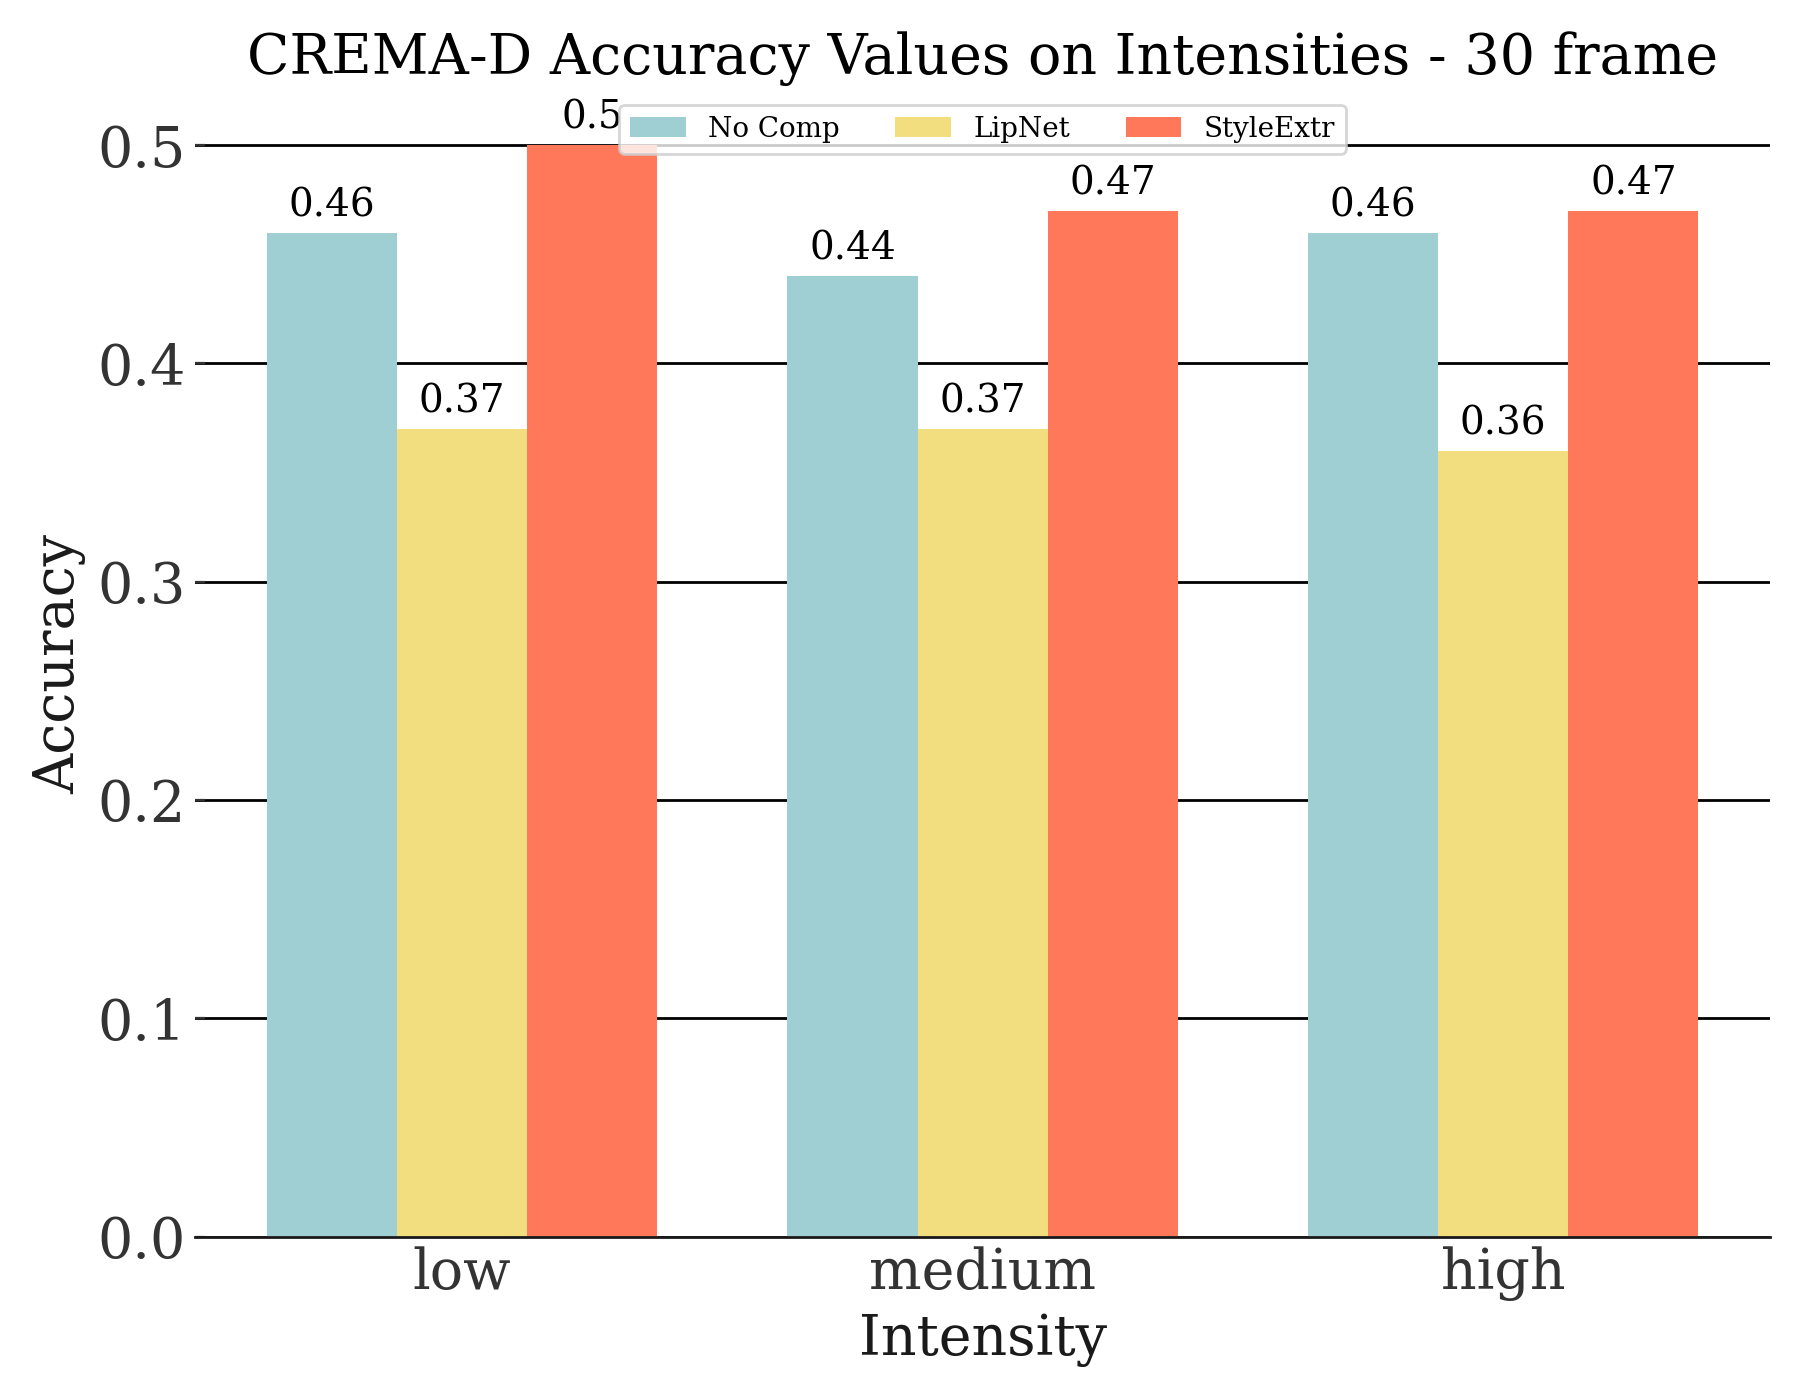
\includegraphics[width=\textwidth]{res/crema-intensities-30.png}
%     \end{subfigure}
%     \begin{subfigure}[b]{0.45\textwidth}
%       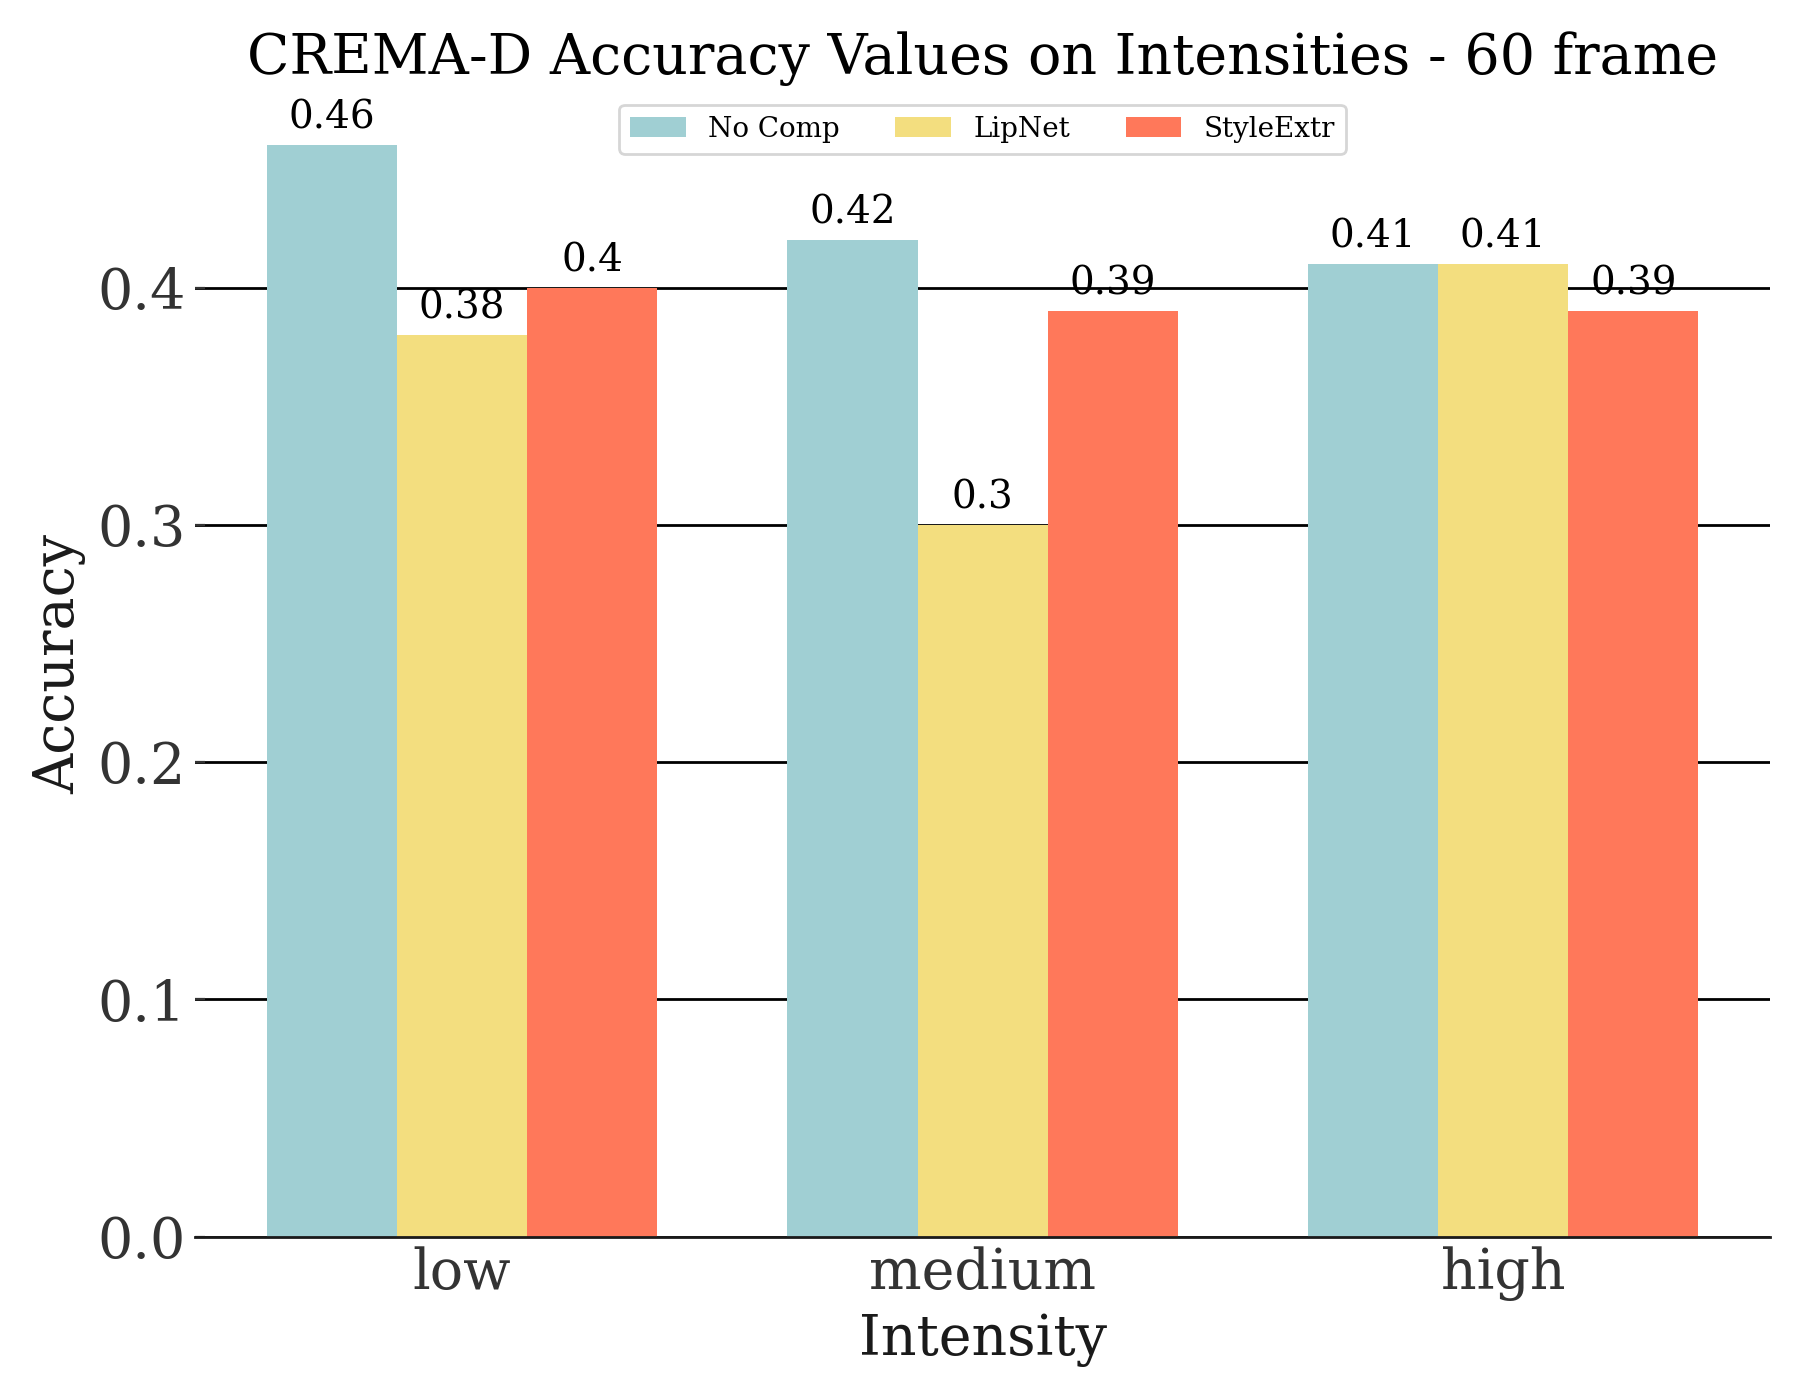
\includegraphics[width=\textwidth]{res/crema-intensities-60.png}
%     \end{subfigure}
%     \caption{Validation accuracies of our models on the CREMA-D corpus depending on the intensity by which the emotions were expressed.}
%     \label{fig:crema_intesities}
% \end{figure}

% \subsection{Phonetic (In-)Dependence}
% In section \ref{sec:human} we already saw that the phonetic performance of existing FER models was low and varied between phonemes. After training our single-frame models, we run the same analysis again to determine the improvements in phonetic performance and to figure out if and how the lexical compensators impact the results.

% We ran the same test as we did in section \ref{sec:human} on the validation set of RAVDESS (Actors 4 and 5) with the models we trained with a frame-window size of one. All three models perform very similarly, struggling and having higher accuracy on the same phonemes. The lexical compensators thus do not increase performance or robustness on a phonetic level.

% We conclude that the lexical compensators, as we implemented them, do not replicate the results of human benchmarking, where our annotators were able to predict the underlying emotions on a similar level of accuracy independent of the phoneme.

% \begin{figure}
%     \centering
%     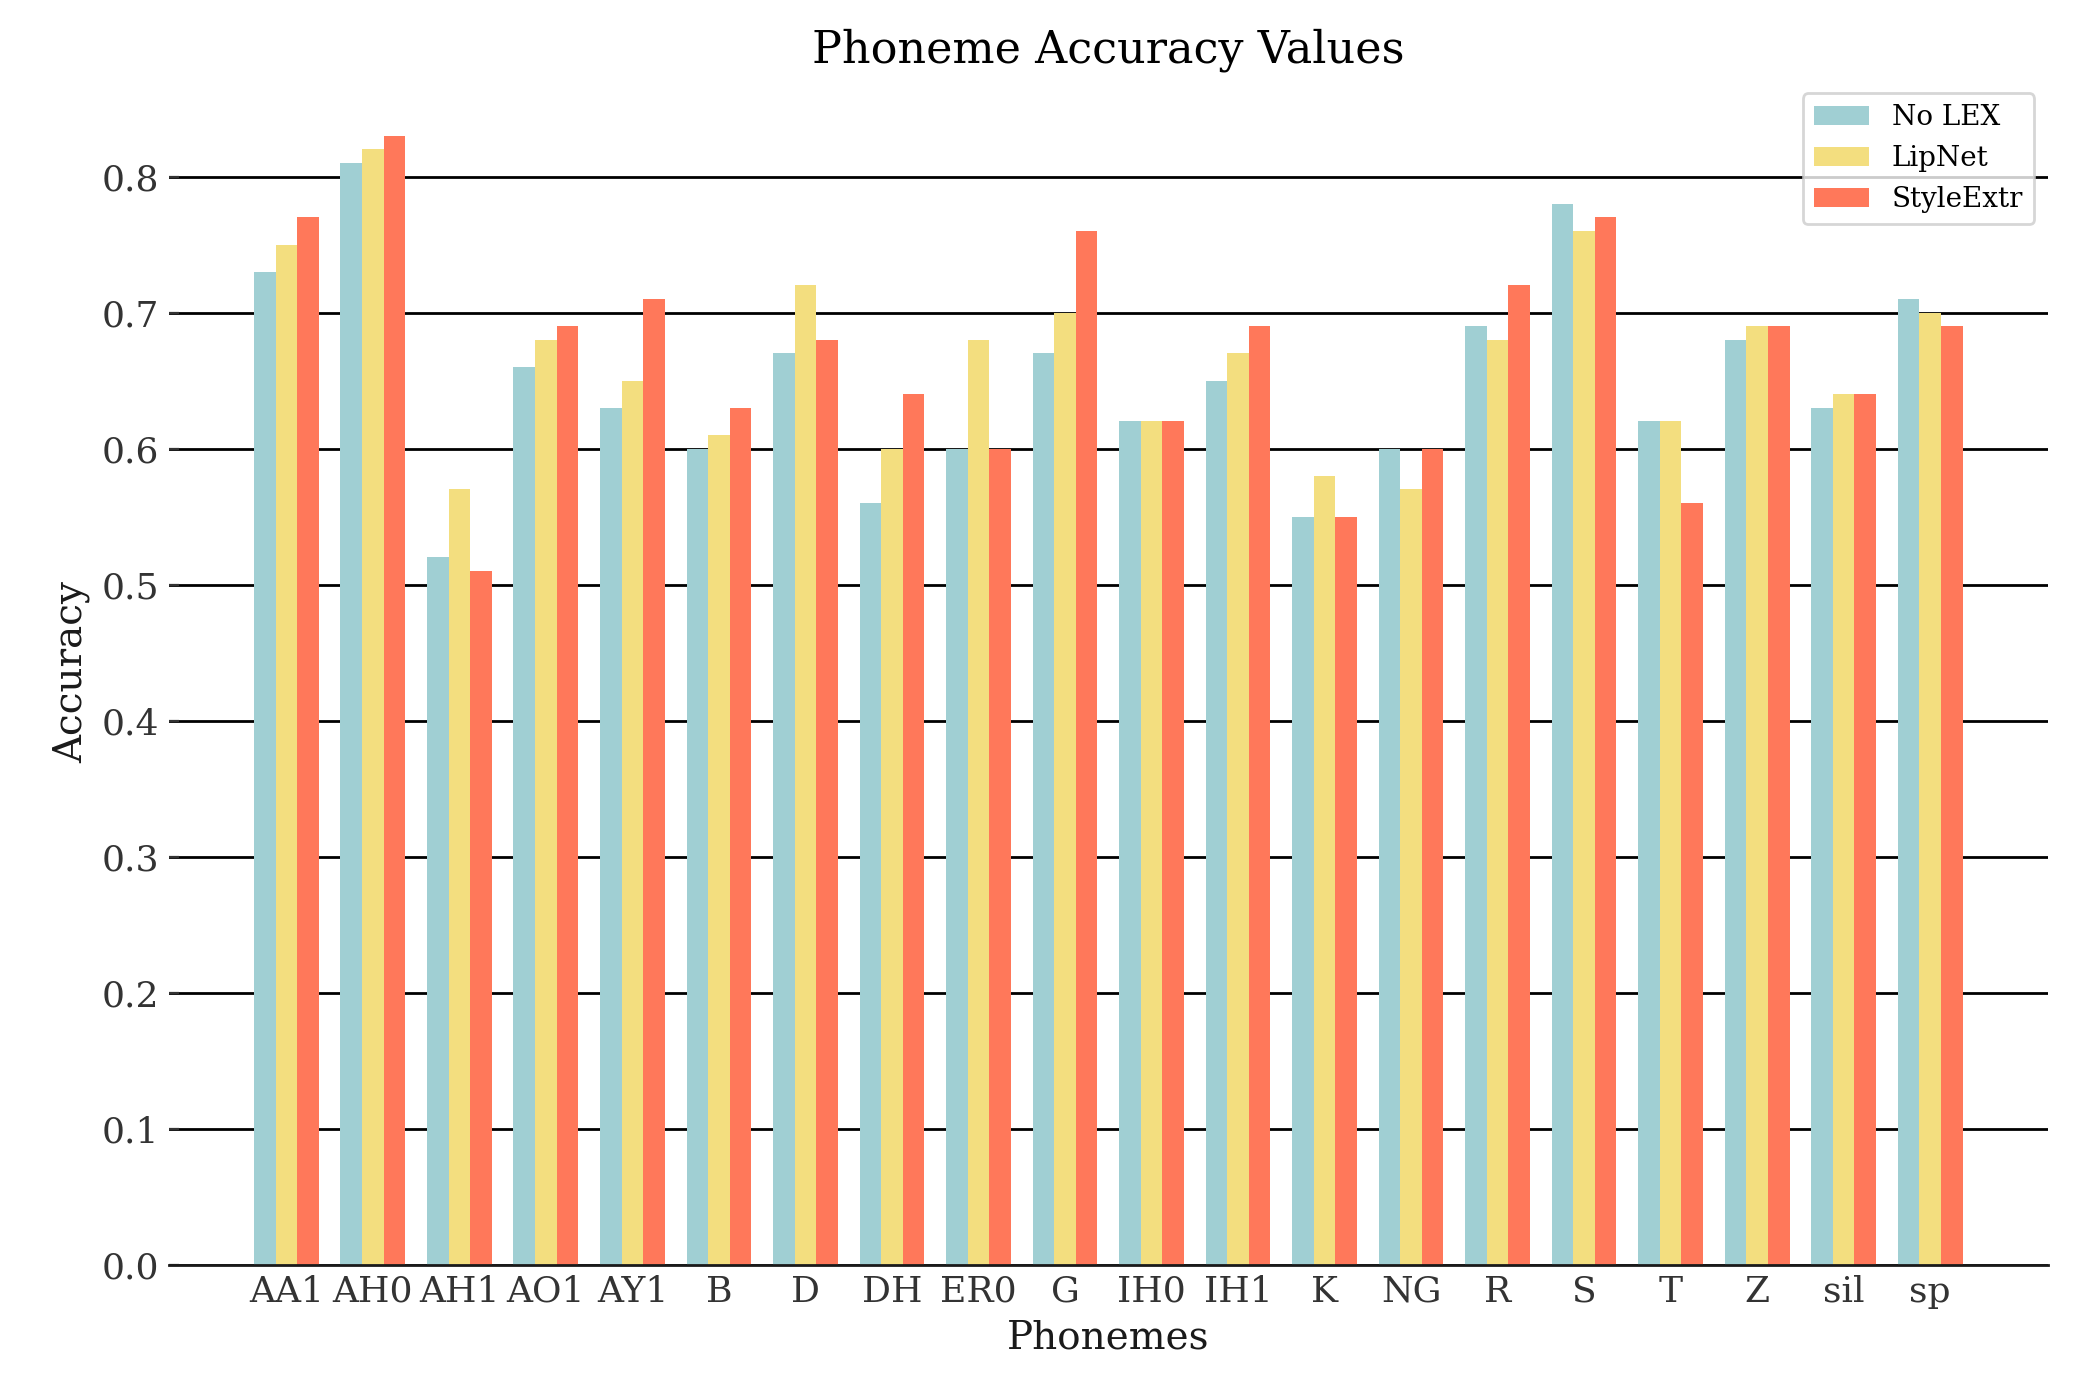
\includegraphics[width=0.8\textwidth]{res/ModelsOnPhones.png}
%     \caption{Evaluating the models we trained with a frame-window size of one based on the phoneme spoken in the frame. There is no significant difference on whether a lexical compensator is used or not.}
%     \label{fig:modelsonphones}
% \end{figure}


% \subsection{Multilingual Datasets}
% \label{sec:multilingual}
% In section \ref{sec:german} we collected samples for a German dataset. We now want to analyse the performance of our models to draw conclusions on their multilingual performance. 

% We validated our models on the videos of the German dataset. The models for 90 frames could not be used since the videos were too short. The general trend from section \ref{sec:cross_dataset} continues. The model without a lexical compensator and the StyleExtractor model perform increasingly better with higher frame-window size. The LipNet models performance does not increase with more temporal information. Compared to the results from section \ref{sec:cross_dataset} there is another decrease in accuracy, of around 10 percentage points. It is however not conclusive if this decrease is due to the language switch or other factors:
% \begin{itemize}
%     \item The recordings are not of the same quality as those of CREMA-D. Due to the recent coronavirus pandemic all recordings had to be done remotely by the actors themselves using the TAWNY recording tool.
%     \item The preparation of the actors were not comparable to those on CREMA-D. We did not have stimuli to actually put the actors into the desired emotional state and relied on their acting ability to convey the emotion.
%     \item The actors only had one take to record their statements. Producers of other datasets generally have the capacity to have multiple takes for each recording.
% \end{itemize}

% \begin{figure}
%     \centering
%     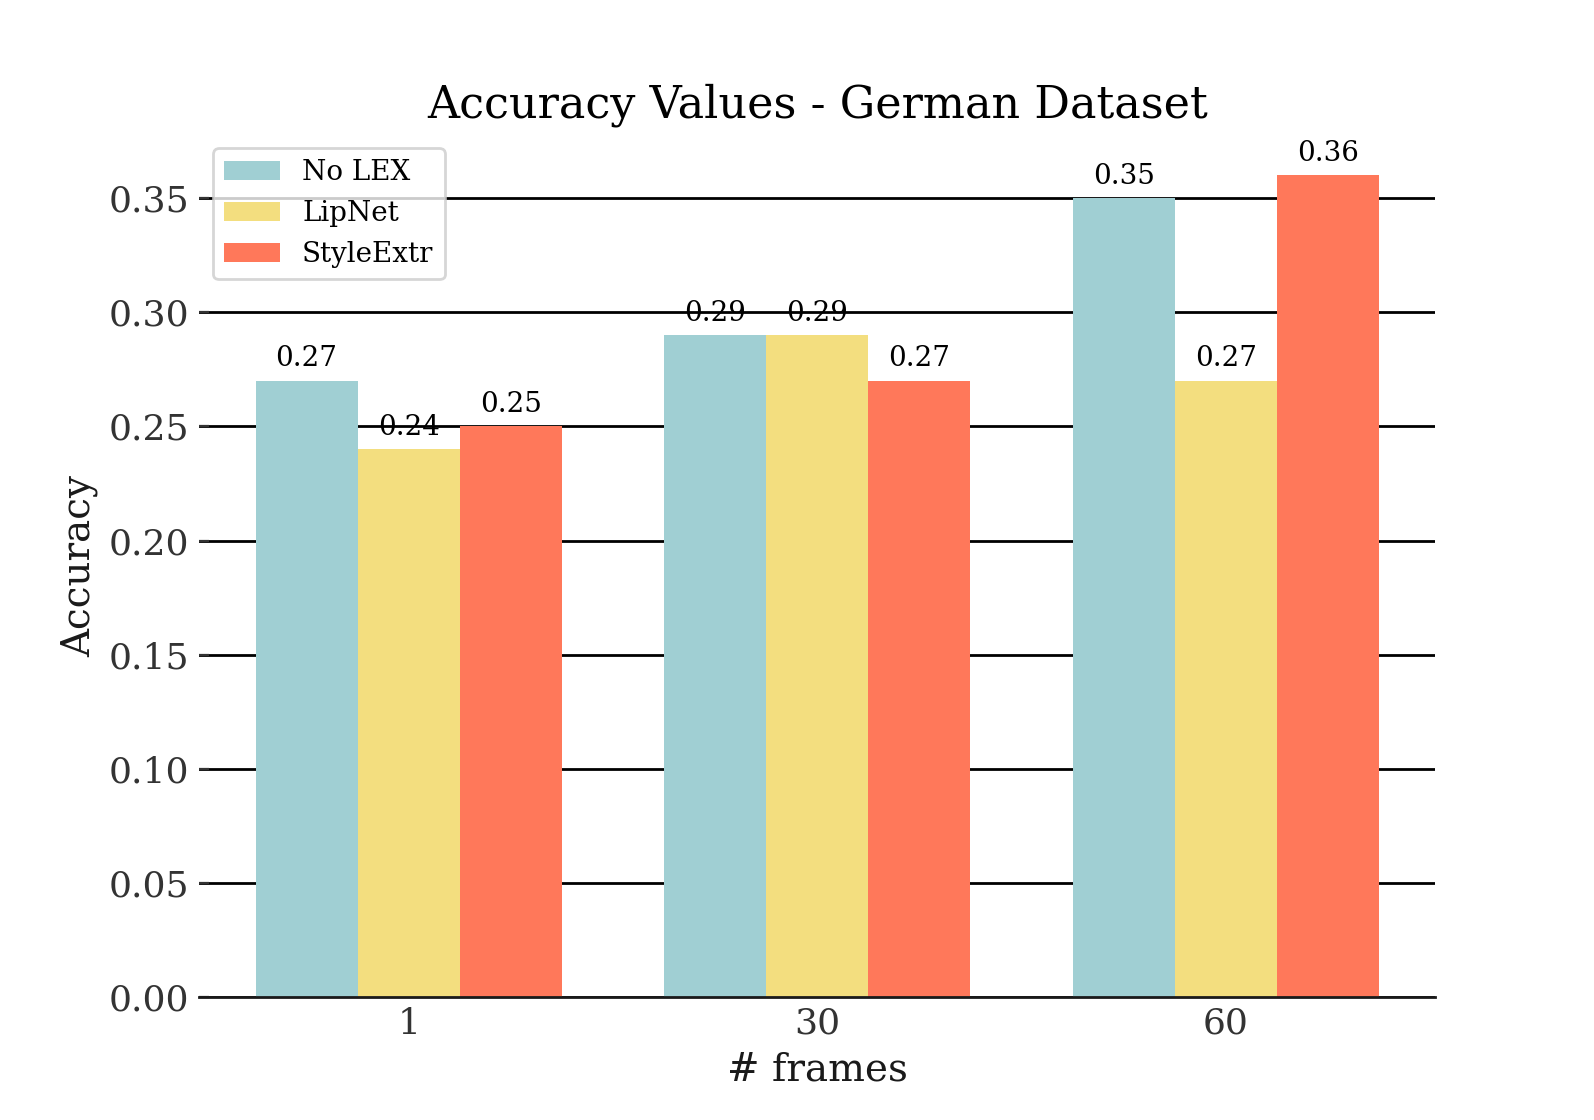
\includegraphics[width=0.8\textwidth]{res/GermanResults.png}
%     \caption{Evaluating the models we trained on the German dataset from section \ref{sec:german}.}
%     \label{fig:german_res}
% \end{figure}

% We can conclude that our models can adapt to recordings in German without much trouble. We would see usable and comparable results with a dataset of another language given similar quality.

% \subsection{Computational Performance}
% \label{sub:computational}
% Strong and robust performance in accuracy is important in FER models, but certainly not the only metric by which we judge them. Other factors, like application range and computational performance are also reasons to use one model over another. We have three different models that are very similar in validation accuracy during training, yet differ when it comes to complexity. The temporalized FER model without any lexical compensator is the easiest model to use. It only requires a facial crop of the image, and has no second input which needs to be preprocessed and predicted during model usage. This also makes it the most computationally performant model. The model using LipNet as its compensator also has easy preprocessing steps, needing an additional crop of the orofacial area. The pruned part of LipNet that we use has 327648 parameters, and does make up a large part of the total network size. While the model with the style extractor has a similar size with 361468 parameters, it also needs to run a FaceMesh preprocessing step for its input.

% \subsection{Real World Application}
% The models we have built have been tested on artificial datasets, where one input video had a specific emotional label. This is not the case in real world scenarios. In those cases our models should be the source of the emotional label, which requires more nuance in predicting the emotions for a given sequence. While our models increase in accuracy with larger frame-window sizes, we need to consider that an emotional expression does not last up to 90 frames, which is three seconds in a video at 30 frames per second. An emotional state that expresses itself in only a small subset of this window might go undetected. In this case, a smaller frame-window size is more beneficial, and a drop in accuracy might have to be taken. As mentioned in section  \ref{sub:computational}, not all models perform similarly based on estimation time. A real-time application might need to prioritise a more efficient model, even though it might not be as accurate.

% Estimations using a temporal model can also be applied using a sliding window approach. The model using 90 frames can analyse a video with a stride of 30 frames, a one second equivalent. This produces overlapping results, which can be further analysed and used for aggregated results.

% The selection of the "right" model depends on the context in which it will be used in. In a scenario where only images are available, it would be required to use one of the single frame models and forego the temporal dimension. Very short clips might also not be able to use the full extend of the temporal dimension. Like we have seen with validating the CREMA-D corpus in section \ref{sec:cross_dataset}, clips with less than 90 frames could not be analysed with the 90-frame model.

% \subsection{Performance on Non-talking Subjects}
